% Created by tikzDevice version 0.10.1 on 2016-08-17 14:40:23
% !TEX encoding = UTF-8 Unicode
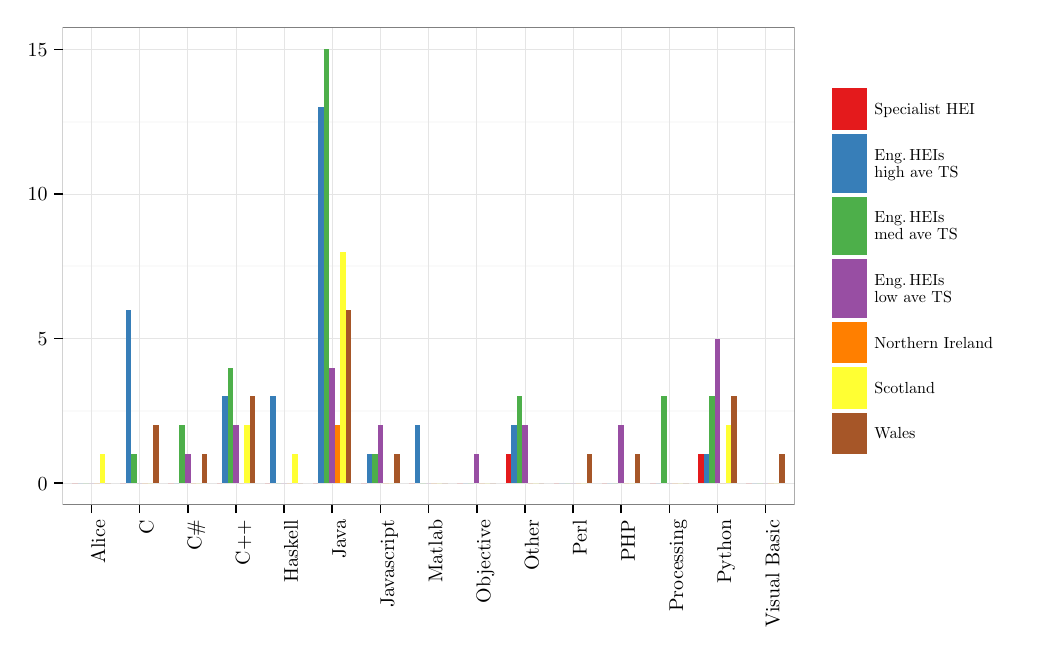
\begin{tikzpicture}[x=1pt,y=1pt]
\definecolor{fillColor}{RGB}{255,255,255}
\path[use as bounding box,fill=fillColor,fill opacity=0.00] (0,0) rectangle (361.35,216.81);
\begin{scope}
\path[clip] (  0.00,  0.00) rectangle (361.35,216.81);
\definecolor{drawColor}{RGB}{255,255,255}
\definecolor{fillColor}{RGB}{255,255,255}

\path[draw=drawColor,line width= 0.6pt,line join=round,line cap=round,fill=fillColor] (  0.00,  0.00) rectangle (361.35,216.81);
\end{scope}
\begin{scope}
\path[clip] ( 12.60, 44.37) rectangle (277.11,216.81);
\definecolor{fillColor}{RGB}{255,255,255}

\path[fill=fillColor] ( 12.60, 44.37) rectangle (277.11,216.81);
\definecolor{drawColor}{gray}{0.98}

\path[draw=drawColor,line width= 0.6pt,line join=round] ( 12.60, 78.34) --
	(277.11, 78.34);

\path[draw=drawColor,line width= 0.6pt,line join=round] ( 12.60,130.59) --
	(277.11,130.59);

\path[draw=drawColor,line width= 0.6pt,line join=round] ( 12.60,182.84) --
	(277.11,182.84);
\definecolor{drawColor}{gray}{0.90}

\path[draw=drawColor,line width= 0.2pt,line join=round] ( 12.60, 52.21) --
	(277.11, 52.21);

\path[draw=drawColor,line width= 0.2pt,line join=round] ( 12.60,104.46) --
	(277.11,104.46);

\path[draw=drawColor,line width= 0.2pt,line join=round] ( 12.60,156.72) --
	(277.11,156.72);

\path[draw=drawColor,line width= 0.2pt,line join=round] ( 12.60,208.97) --
	(277.11,208.97);

\path[draw=drawColor,line width= 0.2pt,line join=round] ( 23.04, 44.37) --
	( 23.04,216.81);

\path[draw=drawColor,line width= 0.2pt,line join=round] ( 40.44, 44.37) --
	( 40.44,216.81);

\path[draw=drawColor,line width= 0.2pt,line join=round] ( 57.84, 44.37) --
	( 57.84,216.81);

\path[draw=drawColor,line width= 0.2pt,line join=round] ( 75.25, 44.37) --
	( 75.25,216.81);

\path[draw=drawColor,line width= 0.2pt,line join=round] ( 92.65, 44.37) --
	( 92.65,216.81);

\path[draw=drawColor,line width= 0.2pt,line join=round] (110.05, 44.37) --
	(110.05,216.81);

\path[draw=drawColor,line width= 0.2pt,line join=round] (127.45, 44.37) --
	(127.45,216.81);

\path[draw=drawColor,line width= 0.2pt,line join=round] (144.85, 44.37) --
	(144.85,216.81);

\path[draw=drawColor,line width= 0.2pt,line join=round] (162.26, 44.37) --
	(162.26,216.81);

\path[draw=drawColor,line width= 0.2pt,line join=round] (179.66, 44.37) --
	(179.66,216.81);

\path[draw=drawColor,line width= 0.2pt,line join=round] (197.06, 44.37) --
	(197.06,216.81);

\path[draw=drawColor,line width= 0.2pt,line join=round] (214.46, 44.37) --
	(214.46,216.81);

\path[draw=drawColor,line width= 0.2pt,line join=round] (231.87, 44.37) --
	(231.87,216.81);

\path[draw=drawColor,line width= 0.2pt,line join=round] (249.27, 44.37) --
	(249.27,216.81);

\path[draw=drawColor,line width= 0.2pt,line join=round] (266.67, 44.37) --
	(266.67,216.81);
\definecolor{fillColor}{RGB}{228,26,28}

\path[fill=fillColor] ( 16.08, 52.21) rectangle ( 18.07, 52.21);
\definecolor{fillColor}{RGB}{55,126,184}

\path[fill=fillColor] ( 18.07, 52.21) rectangle ( 20.06, 52.21);
\definecolor{fillColor}{RGB}{77,175,74}

\path[fill=fillColor] ( 20.06, 52.21) rectangle ( 22.05, 52.21);
\definecolor{fillColor}{RGB}{152,78,163}

\path[fill=fillColor] ( 22.05, 52.21) rectangle ( 24.03, 52.21);
\definecolor{fillColor}{RGB}{255,127,0}

\path[fill=fillColor] ( 24.03, 52.21) rectangle ( 26.02, 52.21);
\definecolor{fillColor}{RGB}{255,255,51}

\path[fill=fillColor] ( 26.02, 52.21) rectangle ( 28.01, 62.66);
\definecolor{fillColor}{RGB}{166,86,40}

\path[fill=fillColor] ( 28.01, 52.21) rectangle ( 30.00, 52.21);
\definecolor{fillColor}{RGB}{228,26,28}

\path[fill=fillColor] ( 33.48, 52.21) rectangle ( 35.47, 52.21);
\definecolor{fillColor}{RGB}{55,126,184}

\path[fill=fillColor] ( 35.47, 52.21) rectangle ( 37.46,114.91);
\definecolor{fillColor}{RGB}{77,175,74}

\path[fill=fillColor] ( 37.46, 52.21) rectangle ( 39.45, 62.66);
\definecolor{fillColor}{RGB}{152,78,163}

\path[fill=fillColor] ( 39.45, 52.21) rectangle ( 41.44, 52.21);
\definecolor{fillColor}{RGB}{255,127,0}

\path[fill=fillColor] ( 41.44, 52.21) rectangle ( 43.42, 52.21);
\definecolor{fillColor}{RGB}{255,255,51}

\path[fill=fillColor] ( 43.42, 52.21) rectangle ( 45.41, 52.21);
\definecolor{fillColor}{RGB}{166,86,40}

\path[fill=fillColor] ( 45.41, 52.21) rectangle ( 47.40, 73.11);
\definecolor{fillColor}{RGB}{228,26,28}

\path[fill=fillColor] ( 50.88, 52.21) rectangle ( 52.87, 52.21);
\definecolor{fillColor}{RGB}{55,126,184}

\path[fill=fillColor] ( 52.87, 52.21) rectangle ( 54.86, 52.21);
\definecolor{fillColor}{RGB}{77,175,74}

\path[fill=fillColor] ( 54.86, 52.21) rectangle ( 56.85, 73.11);
\definecolor{fillColor}{RGB}{152,78,163}

\path[fill=fillColor] ( 56.85, 52.21) rectangle ( 58.84, 62.66);
\definecolor{fillColor}{RGB}{255,127,0}

\path[fill=fillColor] ( 58.84, 52.21) rectangle ( 60.83, 52.21);
\definecolor{fillColor}{RGB}{255,255,51}

\path[fill=fillColor] ( 60.83, 52.21) rectangle ( 62.82, 52.21);
\definecolor{fillColor}{RGB}{166,86,40}

\path[fill=fillColor] ( 62.82, 52.21) rectangle ( 64.80, 62.66);
\definecolor{fillColor}{RGB}{228,26,28}

\path[fill=fillColor] ( 68.29, 52.21) rectangle ( 70.27, 52.21);
\definecolor{fillColor}{RGB}{55,126,184}

\path[fill=fillColor] ( 70.27, 52.21) rectangle ( 72.26, 83.56);
\definecolor{fillColor}{RGB}{77,175,74}

\path[fill=fillColor] ( 72.26, 52.21) rectangle ( 74.25, 94.01);
\definecolor{fillColor}{RGB}{152,78,163}

\path[fill=fillColor] ( 74.25, 52.21) rectangle ( 76.24, 73.11);
\definecolor{fillColor}{RGB}{255,127,0}

\path[fill=fillColor] ( 76.24, 52.21) rectangle ( 78.23, 52.21);
\definecolor{fillColor}{RGB}{255,255,51}

\path[fill=fillColor] ( 78.23, 52.21) rectangle ( 80.22, 73.11);
\definecolor{fillColor}{RGB}{166,86,40}

\path[fill=fillColor] ( 80.22, 52.21) rectangle ( 82.21, 83.56);
\definecolor{fillColor}{RGB}{228,26,28}

\path[fill=fillColor] ( 85.69, 52.21) rectangle ( 87.68, 52.21);
\definecolor{fillColor}{RGB}{55,126,184}

\path[fill=fillColor] ( 87.68, 52.21) rectangle ( 89.67, 83.56);
\definecolor{fillColor}{RGB}{77,175,74}

\path[fill=fillColor] ( 89.67, 52.21) rectangle ( 91.65, 52.21);
\definecolor{fillColor}{RGB}{152,78,163}

\path[fill=fillColor] ( 91.65, 52.21) rectangle ( 93.64, 52.21);
\definecolor{fillColor}{RGB}{255,127,0}

\path[fill=fillColor] ( 93.64, 52.21) rectangle ( 95.63, 52.21);
\definecolor{fillColor}{RGB}{255,255,51}

\path[fill=fillColor] ( 95.63, 52.21) rectangle ( 97.62, 62.66);
\definecolor{fillColor}{RGB}{166,86,40}

\path[fill=fillColor] ( 97.62, 52.21) rectangle ( 99.61, 52.21);
\definecolor{fillColor}{RGB}{228,26,28}

\path[fill=fillColor] (103.09, 52.21) rectangle (105.08, 52.21);
\definecolor{fillColor}{RGB}{55,126,184}

\path[fill=fillColor] (105.08, 52.21) rectangle (107.07,188.07);
\definecolor{fillColor}{RGB}{77,175,74}

\path[fill=fillColor] (107.07, 52.21) rectangle (109.06,208.97);
\definecolor{fillColor}{RGB}{152,78,163}

\path[fill=fillColor] (109.06, 52.21) rectangle (111.04, 94.01);
\definecolor{fillColor}{RGB}{255,127,0}

\path[fill=fillColor] (111.04, 52.21) rectangle (113.03, 73.11);
\definecolor{fillColor}{RGB}{255,255,51}

\path[fill=fillColor] (113.03, 52.21) rectangle (115.02,135.82);
\definecolor{fillColor}{RGB}{166,86,40}

\path[fill=fillColor] (115.02, 52.21) rectangle (117.01,114.91);
\definecolor{fillColor}{RGB}{228,26,28}

\path[fill=fillColor] (120.49, 52.21) rectangle (122.48, 52.21);
\definecolor{fillColor}{RGB}{55,126,184}

\path[fill=fillColor] (122.48, 52.21) rectangle (124.47, 62.66);
\definecolor{fillColor}{RGB}{77,175,74}

\path[fill=fillColor] (124.47, 52.21) rectangle (126.46, 62.66);
\definecolor{fillColor}{RGB}{152,78,163}

\path[fill=fillColor] (126.46, 52.21) rectangle (128.45, 73.11);
\definecolor{fillColor}{RGB}{255,127,0}

\path[fill=fillColor] (128.45, 52.21) rectangle (130.44, 52.21);
\definecolor{fillColor}{RGB}{255,255,51}

\path[fill=fillColor] (130.44, 52.21) rectangle (132.42, 52.21);
\definecolor{fillColor}{RGB}{166,86,40}

\path[fill=fillColor] (132.42, 52.21) rectangle (134.41, 62.66);
\definecolor{fillColor}{RGB}{228,26,28}

\path[fill=fillColor] (137.89, 52.21) rectangle (139.88, 52.21);
\definecolor{fillColor}{RGB}{55,126,184}

\path[fill=fillColor] (139.88, 52.21) rectangle (141.87, 73.11);
\definecolor{fillColor}{RGB}{77,175,74}

\path[fill=fillColor] (141.87, 52.21) rectangle (143.86, 52.21);
\definecolor{fillColor}{RGB}{152,78,163}

\path[fill=fillColor] (143.86, 52.21) rectangle (145.85, 52.21);
\definecolor{fillColor}{RGB}{255,127,0}

\path[fill=fillColor] (145.85, 52.21) rectangle (147.84, 52.21);
\definecolor{fillColor}{RGB}{255,255,51}

\path[fill=fillColor] (147.84, 52.21) rectangle (149.83, 52.21);
\definecolor{fillColor}{RGB}{166,86,40}

\path[fill=fillColor] (149.83, 52.21) rectangle (151.82, 52.21);
\definecolor{fillColor}{RGB}{228,26,28}

\path[fill=fillColor] (155.30, 52.21) rectangle (157.29, 52.21);
\definecolor{fillColor}{RGB}{55,126,184}

\path[fill=fillColor] (157.29, 52.21) rectangle (159.27, 52.21);
\definecolor{fillColor}{RGB}{77,175,74}

\path[fill=fillColor] (159.27, 52.21) rectangle (161.26, 52.21);
\definecolor{fillColor}{RGB}{152,78,163}

\path[fill=fillColor] (161.26, 52.21) rectangle (163.25, 62.66);
\definecolor{fillColor}{RGB}{255,127,0}

\path[fill=fillColor] (163.25, 52.21) rectangle (165.24, 52.21);
\definecolor{fillColor}{RGB}{255,255,51}

\path[fill=fillColor] (165.24, 52.21) rectangle (167.23, 52.21);
\definecolor{fillColor}{RGB}{166,86,40}

\path[fill=fillColor] (167.23, 52.21) rectangle (169.22, 52.21);
\definecolor{fillColor}{RGB}{228,26,28}

\path[fill=fillColor] (172.70, 52.21) rectangle (174.69, 62.66);
\definecolor{fillColor}{RGB}{55,126,184}

\path[fill=fillColor] (174.69, 52.21) rectangle (176.68, 73.11);
\definecolor{fillColor}{RGB}{77,175,74}

\path[fill=fillColor] (176.68, 52.21) rectangle (178.66, 83.56);
\definecolor{fillColor}{RGB}{152,78,163}

\path[fill=fillColor] (178.66, 52.21) rectangle (180.65, 73.11);
\definecolor{fillColor}{RGB}{255,127,0}

\path[fill=fillColor] (180.65, 52.21) rectangle (182.64, 52.21);
\definecolor{fillColor}{RGB}{255,255,51}

\path[fill=fillColor] (182.64, 52.21) rectangle (184.63, 52.21);
\definecolor{fillColor}{RGB}{166,86,40}

\path[fill=fillColor] (184.63, 52.21) rectangle (186.62, 52.21);
\definecolor{fillColor}{RGB}{228,26,28}

\path[fill=fillColor] (190.10, 52.21) rectangle (192.09, 52.21);
\definecolor{fillColor}{RGB}{55,126,184}

\path[fill=fillColor] (192.09, 52.21) rectangle (194.08, 52.21);
\definecolor{fillColor}{RGB}{77,175,74}

\path[fill=fillColor] (194.08, 52.21) rectangle (196.07, 52.21);
\definecolor{fillColor}{RGB}{152,78,163}

\path[fill=fillColor] (196.07, 52.21) rectangle (198.06, 52.21);
\definecolor{fillColor}{RGB}{255,127,0}

\path[fill=fillColor] (198.06, 52.21) rectangle (200.04, 52.21);
\definecolor{fillColor}{RGB}{255,255,51}

\path[fill=fillColor] (200.04, 52.21) rectangle (202.03, 52.21);
\definecolor{fillColor}{RGB}{166,86,40}

\path[fill=fillColor] (202.03, 52.21) rectangle (204.02, 62.66);
\definecolor{fillColor}{RGB}{228,26,28}

\path[fill=fillColor] (207.50, 52.21) rectangle (209.49, 52.21);
\definecolor{fillColor}{RGB}{55,126,184}

\path[fill=fillColor] (209.49, 52.21) rectangle (211.48, 52.21);
\definecolor{fillColor}{RGB}{77,175,74}

\path[fill=fillColor] (211.48, 52.21) rectangle (213.47, 52.21);
\definecolor{fillColor}{RGB}{152,78,163}

\path[fill=fillColor] (213.47, 52.21) rectangle (215.46, 73.11);
\definecolor{fillColor}{RGB}{255,127,0}

\path[fill=fillColor] (215.46, 52.21) rectangle (217.45, 52.21);
\definecolor{fillColor}{RGB}{255,255,51}

\path[fill=fillColor] (217.45, 52.21) rectangle (219.44, 52.21);
\definecolor{fillColor}{RGB}{166,86,40}

\path[fill=fillColor] (219.44, 52.21) rectangle (221.42, 62.66);
\definecolor{fillColor}{RGB}{228,26,28}

\path[fill=fillColor] (224.90, 52.21) rectangle (226.89, 52.21);
\definecolor{fillColor}{RGB}{55,126,184}

\path[fill=fillColor] (226.89, 52.21) rectangle (228.88, 52.21);
\definecolor{fillColor}{RGB}{77,175,74}

\path[fill=fillColor] (228.88, 52.21) rectangle (230.87, 83.56);
\definecolor{fillColor}{RGB}{152,78,163}

\path[fill=fillColor] (230.87, 52.21) rectangle (232.86, 52.21);
\definecolor{fillColor}{RGB}{255,127,0}

\path[fill=fillColor] (232.86, 52.21) rectangle (234.85, 52.21);
\definecolor{fillColor}{RGB}{255,255,51}

\path[fill=fillColor] (234.85, 52.21) rectangle (236.84, 52.21);
\definecolor{fillColor}{RGB}{166,86,40}

\path[fill=fillColor] (236.84, 52.21) rectangle (238.83, 52.21);
\definecolor{fillColor}{RGB}{228,26,28}

\path[fill=fillColor] (242.31, 52.21) rectangle (244.30, 62.66);
\definecolor{fillColor}{RGB}{55,126,184}

\path[fill=fillColor] (244.30, 52.21) rectangle (246.28, 62.66);
\definecolor{fillColor}{RGB}{77,175,74}

\path[fill=fillColor] (246.28, 52.21) rectangle (248.27, 83.56);
\definecolor{fillColor}{RGB}{152,78,163}

\path[fill=fillColor] (248.27, 52.21) rectangle (250.26,104.46);
\definecolor{fillColor}{RGB}{255,127,0}

\path[fill=fillColor] (250.26, 52.21) rectangle (252.25, 52.21);
\definecolor{fillColor}{RGB}{255,255,51}

\path[fill=fillColor] (252.25, 52.21) rectangle (254.24, 73.11);
\definecolor{fillColor}{RGB}{166,86,40}

\path[fill=fillColor] (254.24, 52.21) rectangle (256.23, 83.56);
\definecolor{fillColor}{RGB}{228,26,28}

\path[fill=fillColor] (259.71, 52.21) rectangle (261.70, 52.21);
\definecolor{fillColor}{RGB}{55,126,184}

\path[fill=fillColor] (261.70, 52.21) rectangle (263.69, 52.21);
\definecolor{fillColor}{RGB}{77,175,74}

\path[fill=fillColor] (263.69, 52.21) rectangle (265.68, 52.21);
\definecolor{fillColor}{RGB}{152,78,163}

\path[fill=fillColor] (265.68, 52.21) rectangle (267.66, 52.21);
\definecolor{fillColor}{RGB}{255,127,0}

\path[fill=fillColor] (267.66, 52.21) rectangle (269.65, 52.21);
\definecolor{fillColor}{RGB}{255,255,51}

\path[fill=fillColor] (269.65, 52.21) rectangle (271.64, 52.21);
\definecolor{fillColor}{RGB}{166,86,40}

\path[fill=fillColor] (271.64, 52.21) rectangle (273.63, 62.66);
\definecolor{drawColor}{gray}{0.50}

\path[draw=drawColor,line width= 0.6pt,line join=round,line cap=round] ( 12.60, 44.37) rectangle (277.11,216.81);
\end{scope}
\begin{scope}
\path[clip] (  0.00,  0.00) rectangle (361.35,216.81);
\definecolor{drawColor}{RGB}{0,0,0}

\node[text=drawColor,anchor=base east,inner sep=0pt, outer sep=0pt, scale=  0.72] at (  7.20, 49.73) {0};

\node[text=drawColor,anchor=base east,inner sep=0pt, outer sep=0pt, scale=  0.72] at (  7.20,101.98) {5};

\node[text=drawColor,anchor=base east,inner sep=0pt, outer sep=0pt, scale=  0.72] at (  7.20,154.24) {10};

\node[text=drawColor,anchor=base east,inner sep=0pt, outer sep=0pt, scale=  0.72] at (  7.20,206.49) {15};
\end{scope}
\begin{scope}
\path[clip] (  0.00,  0.00) rectangle (361.35,216.81);
\definecolor{drawColor}{RGB}{0,0,0}

\path[draw=drawColor,line width= 0.6pt,line join=round] (  9.60, 52.21) --
	( 12.60, 52.21);

\path[draw=drawColor,line width= 0.6pt,line join=round] (  9.60,104.46) --
	( 12.60,104.46);

\path[draw=drawColor,line width= 0.6pt,line join=round] (  9.60,156.72) --
	( 12.60,156.72);

\path[draw=drawColor,line width= 0.6pt,line join=round] (  9.60,208.97) --
	( 12.60,208.97);
\end{scope}
\begin{scope}
\path[clip] (  0.00,  0.00) rectangle (361.35,216.81);
\definecolor{drawColor}{RGB}{0,0,0}

\path[draw=drawColor,line width= 0.6pt,line join=round] ( 23.04, 41.37) --
	( 23.04, 44.37);

\path[draw=drawColor,line width= 0.6pt,line join=round] ( 40.44, 41.37) --
	( 40.44, 44.37);

\path[draw=drawColor,line width= 0.6pt,line join=round] ( 57.84, 41.37) --
	( 57.84, 44.37);

\path[draw=drawColor,line width= 0.6pt,line join=round] ( 75.25, 41.37) --
	( 75.25, 44.37);

\path[draw=drawColor,line width= 0.6pt,line join=round] ( 92.65, 41.37) --
	( 92.65, 44.37);

\path[draw=drawColor,line width= 0.6pt,line join=round] (110.05, 41.37) --
	(110.05, 44.37);

\path[draw=drawColor,line width= 0.6pt,line join=round] (127.45, 41.37) --
	(127.45, 44.37);

\path[draw=drawColor,line width= 0.6pt,line join=round] (144.85, 41.37) --
	(144.85, 44.37);

\path[draw=drawColor,line width= 0.6pt,line join=round] (162.26, 41.37) --
	(162.26, 44.37);

\path[draw=drawColor,line width= 0.6pt,line join=round] (179.66, 41.37) --
	(179.66, 44.37);

\path[draw=drawColor,line width= 0.6pt,line join=round] (197.06, 41.37) --
	(197.06, 44.37);

\path[draw=drawColor,line width= 0.6pt,line join=round] (214.46, 41.37) --
	(214.46, 44.37);

\path[draw=drawColor,line width= 0.6pt,line join=round] (231.87, 41.37) --
	(231.87, 44.37);

\path[draw=drawColor,line width= 0.6pt,line join=round] (249.27, 41.37) --
	(249.27, 44.37);

\path[draw=drawColor,line width= 0.6pt,line join=round] (266.67, 41.37) --
	(266.67, 44.37);
\end{scope}
\begin{scope}
\path[clip] (  0.00,  0.00) rectangle (361.35,216.81);
\definecolor{drawColor}{RGB}{0,0,0}

\node[text=drawColor,rotate= 90.00,anchor=base east,inner sep=0pt, outer sep=0pt, scale=  0.72] at ( 28.00, 38.97) {Alice};

\node[text=drawColor,rotate= 90.00,anchor=base east,inner sep=0pt, outer sep=0pt, scale=  0.72] at ( 45.40, 38.97) {C};

\node[text=drawColor,rotate= 90.00,anchor=base east,inner sep=0pt, outer sep=0pt, scale=  0.72] at ( 62.80, 38.97) {C\#};

\node[text=drawColor,rotate= 90.00,anchor=base east,inner sep=0pt, outer sep=0pt, scale=  0.72] at ( 80.20, 38.97) {C++};

\node[text=drawColor,rotate= 90.00,anchor=base east,inner sep=0pt, outer sep=0pt, scale=  0.72] at ( 97.61, 38.97) {Haskell};

\node[text=drawColor,rotate= 90.00,anchor=base east,inner sep=0pt, outer sep=0pt, scale=  0.72] at (115.01, 38.97) {Java};

\node[text=drawColor,rotate= 90.00,anchor=base east,inner sep=0pt, outer sep=0pt, scale=  0.72] at (132.41, 38.97) {Javascript};

\node[text=drawColor,rotate= 90.00,anchor=base east,inner sep=0pt, outer sep=0pt, scale=  0.72] at (149.81, 38.97) {Matlab};

\node[text=drawColor,rotate= 90.00,anchor=base east,inner sep=0pt, outer sep=0pt, scale=  0.72] at (167.22, 38.97) {Objective};

\node[text=drawColor,rotate= 90.00,anchor=base east,inner sep=0pt, outer sep=0pt, scale=  0.72] at (184.62, 38.97) {Other};

\node[text=drawColor,rotate= 90.00,anchor=base east,inner sep=0pt, outer sep=0pt, scale=  0.72] at (202.02, 38.97) {Perl};

\node[text=drawColor,rotate= 90.00,anchor=base east,inner sep=0pt, outer sep=0pt, scale=  0.72] at (219.42, 38.97) {PHP};

\node[text=drawColor,rotate= 90.00,anchor=base east,inner sep=0pt, outer sep=0pt, scale=  0.72] at (236.82, 38.97) {Processing};

\node[text=drawColor,rotate= 90.00,anchor=base east,inner sep=0pt, outer sep=0pt, scale=  0.72] at (254.23, 38.97) {Python};

\node[text=drawColor,rotate= 90.00,anchor=base east,inner sep=0pt, outer sep=0pt, scale=  0.72] at (271.63, 38.97) {Visual Basic};
\end{scope}
\begin{scope}
\path[clip] (  0.00,  0.00) rectangle (361.35,216.81);
\definecolor{fillColor}{RGB}{255,255,255}

\path[fill=fillColor] (285.65, 57.75) rectangle (352.81,203.43);
\end{scope}
\begin{scope}
\path[clip] (  0.00,  0.00) rectangle (361.35,216.81);
\definecolor{fillColor}{RGB}{228,26,28}

\path[fill=fillColor] (290.63,179.85) rectangle (303.43,194.83);
\end{scope}
\begin{scope}
\path[clip] (  0.00,  0.00) rectangle (361.35,216.81);
\definecolor{fillColor}{RGB}{55,126,184}

\path[fill=fillColor] (290.63,157.22) rectangle (303.43,178.43);
\end{scope}
\begin{scope}
\path[clip] (  0.00,  0.00) rectangle (361.35,216.81);
\definecolor{fillColor}{RGB}{77,175,74}

\path[fill=fillColor] (290.63,134.59) rectangle (303.43,155.80);
\end{scope}
\begin{scope}
\path[clip] (  0.00,  0.00) rectangle (361.35,216.81);
\definecolor{fillColor}{RGB}{152,78,163}

\path[fill=fillColor] (290.63,111.96) rectangle (303.43,133.17);
\end{scope}
\begin{scope}
\path[clip] (  0.00,  0.00) rectangle (361.35,216.81);
\definecolor{fillColor}{RGB}{255,127,0}

\path[fill=fillColor] (290.63, 95.55) rectangle (303.43,110.54);
\end{scope}
\begin{scope}
\path[clip] (  0.00,  0.00) rectangle (361.35,216.81);
\definecolor{fillColor}{RGB}{255,255,51}

\path[fill=fillColor] (290.63, 79.14) rectangle (303.43, 94.13);
\end{scope}
\begin{scope}
\path[clip] (  0.00,  0.00) rectangle (361.35,216.81);
\definecolor{fillColor}{RGB}{166,86,40}

\path[fill=fillColor] (290.63, 62.73) rectangle (303.43, 77.72);
\end{scope}
\begin{scope}
\path[clip] (  0.00,  0.00) rectangle (361.35,216.81);
\definecolor{drawColor}{RGB}{0,0,0}

\node[text=drawColor,anchor=base west,inner sep=0pt, outer sep=0pt, scale=  0.58] at (305.95,191.58) {};

\node[text=drawColor,anchor=base west,inner sep=0pt, outer sep=0pt, scale=  0.58] at (305.95,185.36) {Specialist HEI};

\node[text=drawColor,anchor=base west,inner sep=0pt, outer sep=0pt, scale=  0.58] at (305.95,179.14) {};
\end{scope}
\begin{scope}
\path[clip] (  0.00,  0.00) rectangle (361.35,216.81);
\definecolor{drawColor}{RGB}{0,0,0}

\node[text=drawColor,anchor=base west,inner sep=0pt, outer sep=0pt, scale=  0.58] at (305.95,175.17) {};

\node[text=drawColor,anchor=base west,inner sep=0pt, outer sep=0pt, scale=  0.58] at (305.95,168.95) {Eng.\,HEIs};

\node[text=drawColor,anchor=base west,inner sep=0pt, outer sep=0pt, scale=  0.58] at (305.95,162.73) {high ave TS};

\node[text=drawColor,anchor=base west,inner sep=0pt, outer sep=0pt, scale=  0.58] at (305.95,156.51) {};
\end{scope}
\begin{scope}
\path[clip] (  0.00,  0.00) rectangle (361.35,216.81);
\definecolor{drawColor}{RGB}{0,0,0}

\node[text=drawColor,anchor=base west,inner sep=0pt, outer sep=0pt, scale=  0.58] at (305.95,152.54) {};

\node[text=drawColor,anchor=base west,inner sep=0pt, outer sep=0pt, scale=  0.58] at (305.95,146.32) {Eng.\,HEIs};

\node[text=drawColor,anchor=base west,inner sep=0pt, outer sep=0pt, scale=  0.58] at (305.95,140.10) {med ave TS};

\node[text=drawColor,anchor=base west,inner sep=0pt, outer sep=0pt, scale=  0.58] at (305.95,133.88) {};
\end{scope}
\begin{scope}
\path[clip] (  0.00,  0.00) rectangle (361.35,216.81);
\definecolor{drawColor}{RGB}{0,0,0}

\node[text=drawColor,anchor=base west,inner sep=0pt, outer sep=0pt, scale=  0.58] at (305.95,129.91) {};

\node[text=drawColor,anchor=base west,inner sep=0pt, outer sep=0pt, scale=  0.58] at (305.95,123.69) {Eng.\,HEIs};

\node[text=drawColor,anchor=base west,inner sep=0pt, outer sep=0pt, scale=  0.58] at (305.95,117.47) {low ave TS};

\node[text=drawColor,anchor=base west,inner sep=0pt, outer sep=0pt, scale=  0.58] at (305.95,111.25) {};
\end{scope}
\begin{scope}
\path[clip] (  0.00,  0.00) rectangle (361.35,216.81);
\definecolor{drawColor}{RGB}{0,0,0}

\node[text=drawColor,anchor=base west,inner sep=0pt, outer sep=0pt, scale=  0.58] at (305.95,107.28) {};

\node[text=drawColor,anchor=base west,inner sep=0pt, outer sep=0pt, scale=  0.58] at (305.95,101.06) {Northern Ireland};

\node[text=drawColor,anchor=base west,inner sep=0pt, outer sep=0pt, scale=  0.58] at (305.95, 94.84) {};
\end{scope}
\begin{scope}
\path[clip] (  0.00,  0.00) rectangle (361.35,216.81);
\definecolor{drawColor}{RGB}{0,0,0}

\node[text=drawColor,anchor=base west,inner sep=0pt, outer sep=0pt, scale=  0.58] at (305.95, 90.87) {};

\node[text=drawColor,anchor=base west,inner sep=0pt, outer sep=0pt, scale=  0.58] at (305.95, 84.65) {Scotland};

\node[text=drawColor,anchor=base west,inner sep=0pt, outer sep=0pt, scale=  0.58] at (305.95, 78.43) {};
\end{scope}
\begin{scope}
\path[clip] (  0.00,  0.00) rectangle (361.35,216.81);
\definecolor{drawColor}{RGB}{0,0,0}

\node[text=drawColor,anchor=base west,inner sep=0pt, outer sep=0pt, scale=  0.58] at (305.95, 74.46) {};

\node[text=drawColor,anchor=base west,inner sep=0pt, outer sep=0pt, scale=  0.58] at (305.95, 68.24) {Wales};

\node[text=drawColor,anchor=base west,inner sep=0pt, outer sep=0pt, scale=  0.58] at (305.95, 62.02) {};
\end{scope}
\end{tikzpicture}
